\documentclass[11pt]{article}
\usepackage{amssymb}
\usepackage{amsmath}
\usepackage{pdfpages}
\usepackage{graphicx}
\usepackage[authoryear,round]{natbib}
\usepackage{algorithm,algorithmic}
\bibliographystyle{plainnat}
\usepackage{color}
\usepackage{graphicx}
\newtheorem{theorem}{Theorem}
\newtheorem{lemma}[theorem]{Lemma}
\newtheorem{corollary}[theorem]{Corollary}
\newtheorem{conjecture}[theorem]{Conjecture}
\newtheorem{definition}{Definition}
\usepackage{xspace}
\usepackage{paralist}
\usepackage{setspace}
\textwidth 6.5in
\textheight 10in
\hoffset -1in
\voffset -1.4in
\singlespacing
\parindent 0em
\parskip .4em
% Abbreviations
\newcommand{\otol}{Open Tree of Life\xspace}
\newcommand{\ps}{phylogenetic statement\xspace}
\newcommand{\pss}{phylogenetic statements\xspace}
\newcommand{\PSs}{Phylogenetic Statements\xspace}
\newcommand{\PS}{Phylogenetic Statement\xspace}
\newcommand{\SWIPSD}{Sum of Weighted Input \PSs Displayed\xspace}
\newcommand{\MSWIPSD}{Maximum \SWIPSD \xspace}
\newcommand{\newick}[1]{\texttt{#1}\xspace}
\newcommand{\otc}[0]{\texttt{otcetera}\xspace}
\newcommand{\otcprune}[0]{\texttt{otc-prune-taxonomy}\xspace}
\newcommand{\otcdecompose}[0]{\texttt{otc-uncontested-decompose}\xspace}
\newcommand{\nexson}[0]{\texttt{otNexSON}\xspace}
\newcommand{\gcmdr}[0]{\texttt{gcmdr}\xspace}
\newcommand{\simplification}[0]{\\\noindent\textsc{Simplification Action(s)}:\xspace}
\newcommand{\undoActions}[0]{\\\noindent\textsc{``Undo'' Simplification Action(s)}:\xspace}
\newcommand{\stepExplanation}[0]{\\\noindent\textsc{Explanation}:\xspace}
\newcommand{\stepInput}[0]{\\\noindent\textsc{Input}:\xspace}
\newcommand{\stepOutput}[0]{\\\noindent\textsc{Output}:\xspace}
\newcommand{\currImpl}[0]{\\\noindent\textsc{Current Impl.}:\xspace}
\newcommand{\implTODO}[0]{\\\noindent\textsc{TODO for Impl.}:\xspace}
\newcommand{\currURL}[0]{\\\noindent\textsc{URL for output}:\xspace}
\newcommand{\comment}[1]{{\color{red} \textsc{#1}}\xspace}
\newcommand{\TODO}[1]{\comment{TODO: #1}}
\newcommand{\NeedsAlgorithmicWork}{{\comment{This needs algorithmic work.}}}
\newcommand{\ProofWriteupNeeded}{{\comment{Need to write up this proof}}}

\newcommand{\incLSSS}{Include-LeafSet support statement\xspace}
\newcommand{\incLSSSs}{Include-LeafSet support statements\xspace}

% Notation
\newcommand{\pssInOptimalTree}{\ensuremath{\hat{\mathcal{G}}}\xspace}
\newcommand{\pssFrom}[1]{\ensuremath{\mathcal{G}(#1)}\xspace}
\newcommand{\tripleSetInOptimal}{\ensuremath{\hat{\mathcal{R}}}\xspace}
\newcommand{\leafLabels}[1]{\ensuremath{\mathcal{L}(#1)}}
\newcommand{\parent}[1]{\mbox{parent}(#1)}
\newcommand{\children}[1]{\mbox{children}(#1)}
\newcommand{\nodes}[1]{\mbox{nodes}(#1)}
\newcommand{\treeRoot}[1]{\mbox{root}(#1)}
\newcommand{\taxonomy}[0]{\ensuremath{\mathbb{T}}\xspace}
\newcommand{\prunedTaxonomy}[0]{\ensuremath{\mathbb{T}_P}\xspace}
\newcommand{\phyloInputs}[0]{\ensuremath{\mathcal{T}}}
\newcommand{\expandedPhylo}[0]{\ensuremath{\mathcal{T}_{E}}\xspace}
\newcommand{\prunedSummary}[0]{\ensuremath{\mathcal{S}_{P}}\xspace}
\newcommand{\summaryTree}[0]{\ensuremath{\mathcal{S}}\xspace}
% verbatim, verbatim notation for a \ps
\newcommand{\vvps}[2]{\ensuremath{{#1}\downarrow{#2}}}
% leaf set, verbatim notation for a \ps
\newcommand{\lvps}[2]{\ensuremath{\leafLabels{#1}\downarrow{#2}}}
\newcommand{\leafComp}[2]{\ensuremath{\widetilde{\mathcal{L}_{#2}}\left({#1}\right)}}
\newcommand{\displaysPred}[2]{\ensuremath{\mathbb{I}_d(#1, #2)}}

\newcommand{\leafDes}[1]{\ensuremath{\mathcal{L}_d(#1)}}
\newcommand{\excLeafDes}[1]{\ensuremath{\mathcal{L}_e(#1)}}
%\newcommand{\children}[1]{\ensuremath{\mathcal{C}(#1)}}

\newcommand{\mrca}[2]{\ensuremath{\mbox{mrca}(#1, #2)}}
\newcommand{\treeOf}[1]{\ensuremath{\mbox{tree}(#1)}}
\newcommand{\leafSet}[1]{\leafLabels{#1}}}
\newcommand{\cLeafSet}[1]{\texttt{{#1}.leafLSet}}}
\newcommand{\cDes}[1]{\texttt{{#1}.desIds}}}

\newcommand{\supportingPSSetFull}[2]{\ensuremath{\mbox{\texttt{SuppStatementSet}}[#1, #2]}}
\newcommand{\supportingPSSet}[1]{\ensuremath{\mbox{\texttt{SSS}}[#1]}}
\DeclareMathOperator*{\argmax}{\arg\!\max}

\newcommand{\mthcomment}[1]{{\color{red} #1}\xspace}
\newcommand{\registration}[3]{{\ensuremath{r(#1)=\{#2\}\mid\{#3\}}}\xspace}
\newcommand{\mrcaDesig}[3]{{\ensuremath{m(#1)=\mbox{MRCA}(#2, #3)}}\xspace}
\newcommand{\nodeLinkRot}{Node Link Rot Problem\xspace}
\newcommand{\ottIdInterpretation}{OTT ID Interpretation Problem\xspace}
\newcommand{\fragileOTUMapping}{Fragile OTU Mapping Problem\xspace}

\usepackage{hyperref}
\hypersetup{backref,  linkcolor=blue, citecolor=black, colorlinks=true, hyperindex=true}
\begin{document}
The source for this in the doc subdirectory of the otcetera
    repo \url{https://github.com/mtholder/otcetera/tree/master/doc}.
\begin{center}
    {\bf Proposals for node identification systems in the Open Tree of Life project} \\
{Mark T.~Holder$^{1,2,\ast}$. feel free to contribute and add your name}
\end{center}
This doc really has nothing to do with otcetera, MTH just wanted a spot to
put a \LaTeX doc on this subject, and this repo had a convenient template.

\tableofcontents
\section{Motivation and Requirements}
\subsection{\nodeLinkRot}
As of November 2015 nodes in the synthetic tree are identified in API calls
    using unstable neo4j node IDs.
If these node IDs resolve across versions of the synthetic tree, they will be
    resolving to an arbitrary spot in the synthetic tree.
This will be referred to as the \nodeLinkRot problem in this doc.
Node IDs show up in URLs (some of which users may be in users' bookmarks, hence
    are out of our control) and in our commenting system (feedback repo on GitHub).

\subsection{\ottIdInterpretation}
We also have IDs for taxa in our reference taxonomy, OTT.
That taxonomy is created by rule-based merging of multiple source taxonomies and
    a set of ``patch files.''
The system for deciding when a taxon has changed enough to merit a different OTT ID
    is automated, but not described in user-facing documentation.
In other words, we have not made any promises to people about what these IDs mean.
However, at some point, inquiring minds want to know what the rules are for when
  the OTT IDs will be stable and when they won't.

This is a very minor concern, compared to the other problems mentioned in this section,
  but any solution to the other problems is going to affect what we can say 
  about OTT ID stability and meaning.

\subsection{\fragileOTUMapping}
A primary motivation of our phylesystem corpus of studies, was to enable
  mapping OTUs in published trees to a common taxonomy.
When a curator chooses a taxonomic name, the NexSON representation of the study
  retains the OTT ID and the OTT taxon name.
With a high degree of probability, we can state that the vast majority of the 
  OTU mapping has been name-based (rather than by looking at the inclusion
    sets of OTT and choosing the most appropriate OTT ID).

Currently the name is not guaranteed to remain fixed with that OTT ID, and the
  names are not guaranteed to be unique.
Thus, the stored OTU mapping can become internally inconsistent when OTT is updated.
Note that: (a) we do have a ``uniqname'' field for taxa that have homonyms, and (b)
  new versions of OTT have a file of ``forwarding'' statements for many IDs that 
  are removed from the system.

Since flux in OTT IDs is mainly at the internal taxa, and relatively few of these
  are mapped to OTUs in studies, this is a relatively low level problem.
But it would be nice to have an automatic solution that does not involve sleuthing
  through old versions of OTT.

\subsection{Summary of Requirements}
We would like to accelerate the rate of producing new synthetic trees.
That would exacerbate the problems with node-base URLs.

Any proposal for a system of generating node IDs would have to describe:
\begin{compactenum}
  \item how the
    set of these IDs gets updated when a new version of the synthetic tree or taxonomy are produced,
  \item how the proposal would solve/mediat the \nodeLinkRot), 
  \item how the proposal affects the \fragileOTUMapping, and
  \item what we can promise users of Open Tree about these IDs (the \ottIdInterpretation)
\end{compactenum}

\subsection{Other features that might be nice to have}
\begin{compactenum}
  \item It would be nice to be able to answer questions like ``how long has this grouping
been in the synthetic tree?'' or ``what version of the tree did this grouping first appear?)''
  for groups that are not named.
  This would require some nice definition of taxon concept to stand in for ``this grouping'' in these questions.
  \item One might want a taxon concept that can describe where to place an annotation on a tree.
  Notes: see \href{https://docs.google.com/document/d/1MbiQwy5ImaWUzzCudmkLwKj82oe-QC__e5krsQJ8umE/edit}{hackathon annotations docs} and footnote
  \footnote{
  It seems (to MTH) that it is unlikely that we could reuse a specfic description
    of what properties a group must have before one applies an annotation to it.
  In other words it seems like if the target of annotations is explicitly stated,
    then it will probably only apply to that one property.
  If it is vaguely stated, then it does not seem that worthwhile.
  In short, MTH sees this annotation-transferring use case as a pretty poor
    match for a system of general node identification}.
\end{compactenum}

%%%%%%%%%%%%%%%%%%%%%%%%%%%%%%%%%%%%%%%%%%%%%%%%%%%%%%%%%%%%%%%%%
\section{Proposals}
\subsection{Sampling of inclusions and exclusions}
\subsubsection{Brief summary}
See \href{https://docs.google.com/document/d/1hJHjMckLywnoBuY1xG3I0hP-rsl4l8du3iA8kflEOQE/edit#}{JAR's note on the node ID registry google doc}, the 
\href{https://github.com/OpenTreeOfLife/reference-taxonomy/blob/registry/registry/README.md}{README} in the registry implementation,
and the \href{https://rawgit.com/OpenTreeOfLife/reference-taxonomy/registry/registry/doc/scenarios.html}{``scenarios'' web page} for 
a full description.

The following is based partially on the docs above and partly on slack conversations.

\subsubsection{Some principles}
\begin{compactenum}
  \item OTT IDs of terminal taxa are the ``atomic'' units of an internal node registrations
  \item an internal node registration consists of:
  \begin{compactitem}
    \item an inclusion set: some (but usually not all) descendant terminal taxa IDs, and
    \item an exclusion set: some (but not all) terminal taxa that are not in the clade.
  \end{compactitem}
  \item internal node registrations maintain some flexibility by being interpreted as ``a 
  common ancestor'' of the inclusion set rather than the ``most recent common 
  ancestor'' (e.g a ``node-based'' name) or ``the largest clade that is the 
  ancestor of all of the inclusion set and none of the exclusion set'' (a stem-based name).
  \item The number of included descendants, $y$, and the number of excluded taxa, $x$, will
    be decided based on testing their effects (based on previous revisions.) JAR has some
    results, but you can get the gist of the proposal without knowing those details.
\end{compactenum}

This sample-based registry is, essentially, a collection of automatically
  generated taxon concepts.

\subsubsection{Procedure}
\begin{compactenum}
  \item From the current (and possibly previous) version(s) of OTT,
  we create an initial set of internal node registrations -- one for each internal node in OTT.
  For this initial operation only, the OTT ID becomes the registration ID.
  \begin{compactitem}
    \item The $y$ sampled terminals are chosen by including walking through $y$ distinct
    children of the taxon in OTT.
    Thus if a taxon in OTT has five subtaxa and $y=4$ then a representative from
    4 distinct subtaxa will be chosen.
    In other words, the terminal sampling is ``overdispersed'' compared to random sampling.
    If the number of children is less than the sampling number, then some subtrees will be represented by multiple descendants.
    \item Choosing a terminal OTT ID that is mentioned in multiple source taxonomies increases
    the stability of the system by avoiding potentially problematic/questionable
    taxa from serving as the exemplars in a registration definition.
  \end{compactitem}
  \item Whenever a new version synthetic tree is produced:
    \begin{compactenum}
      \item existing internal node registrations are used to decorate the
      internal nodes of the tree.
      \item If an internal node of the tree lacks any registration, then a new registration is
      created to identify it.
      \item If an internal node of the tree, $Y$, has been assigned multiple registrations:
      \begin{compactenum}
        \item If some of the node registrations map only to $Y$, then this set
          of registrations uniquely identify the node. No new registrations are
          needed.
        \item If {\em none} of the nodes map to $Y$ alone, then a new
        registration is created to identify $Y$.
      \end{compactenum}
      \item What happens if a registration that is associate with a taxonomic name maps to
      multiple nodes in the tree, but each of those nodes also has a different registration
      which uniquely identifies the node? I'm not sure if there is some mechanism to 
      disambiguate any ``taxonomic registrations'' (registrations that are associated with
      a taxonomic name in OTT).
    \end{compactenum}
  \item OTT updates are handled in the same way as synthetic tree updates.
\end{compactenum}
\subsubsection{Concerns}
\begin{compactenum}
  \item exacerbates the \fragileOTUMapping.
  As mentioned \href{https://docs.google.com/document/d/1hJHjMckLywnoBuY1xG3I0hP-rsl4l8du3iA8kflEOQE/edit?pli=1#heading=h.aqib3hn3t8nx}{here},
  the sampling proposal will increase the rate of breaking the connection
  between internal OTT Taxon names and OTT IDs by a factor of 15 (note also that
  most tips in phylesytem trees are mapped to terminals in OTT).
  \item Note that the creation of new synthetic tree can break the association b
  between an OTT ID and an OTT taxonomic name in this system.
  So we would need to alert curators of changes in the interpretations of 
  mappings more frequently than with every OTT update.
  \item It is not clear how we can assign ``higher'' taxonomic names to the 
  synthetic tree in a way that won't be confusing (or at least require a lot
  of software infrastructure to explain).
  It seems inevitable that users will interpret a taxonomic name as meaning
  that the meaning of the name can be discerned by looking at OTT and saying
  the clade includes ``all of the OTT IDs that descend from this taxon in OTT, 
  and no others.''
  But the registration that provides the ID for that OTT taxon name may have a
    looser definition.
\end{compactenum}

\subsection{Name-based OTT IDs. Synthetic tree nodes designated by MRCA of two descendants}
\subsubsection{Procedure}
Reuse the OTT IDs whenever the uniqname has not changed.

Internal nodes in the synthetic tree get designations (instead of true IDs).
These designations use some syntactic trick to concatenate
  a pair of OTT IDs for terminal descendants which point to the node via an MRCA statement.

Retrieval of a node based on an exact designation match would be a very fast look up
  in an index in treemachine-LITE.
If no node a new tree was decorated with that specific designation, we can still
  find a node provided that the two descendants are still in the tree by using
  the MRCA query in the API.

{\bf Note:} an easy method for producing designations that are likely to get reused:
We could produce ``canonical'' pairs of descendants for the MRCA statements
  via a procedure such as:
\begin{compactenum}
  \item At each internal node, sort the child branch order based on the lowest OTT ID (or via a pair of numbers. The first is some score 
  for the OTT ID that captures reliability based on number of source taxonomies
  that include the source, and the second is the numeric interpretation of the OTT ID.
  The second element is used to break ties in a consistent way) 
  \item use the best scoring OTT ID of the first child and the second child to designate the internal node
\end{compactenum}
As long as we assign high numbers for new OTT Ids, then would probably result in
  lots of reuse of which designators are chosen.
This would help us by giving us ``hits'' when we use node IDs

\subsubsection{Pros}
\begin{compactenum}
  \item Easy to implement:
  The current synthetic tree APIs require the server to be able to handle MRCA
    queries, so this is not a new burden.
  \item Slows the divergence of OTT taxon name fields in NexSON from the OTT ID fields in NexSON files.
  \item Would stop a lot of the 404's (or random resolutions) when we update the
  synth tree. It would even be pretty trivial to create a redirect table for cases
  when we know that one of our designators has been merged or removed from OTT.
\end{compactenum}


\subsubsection{Cons}
\begin{compactenum}
  \item Internal OTT IDs are not tied to the internal node designations, which might surprise
  some users.
  \item The fact that the OTT IDs don't mean anything other than ``a taxon that some
  some source has given this name to'' is unfortunate, because that meaning is so 
  semantically impoverished.
  For example, feedback issues could refer some feature of a named taxon, but in 
    a subsequent version of the tree that name may refer to a different set of 
    descendants.
  However,
  \begin{compactenum}
    \item it is fairly easy to explain cases to users the idea that OTT ID is stable,
    but it corresponds to different set of taxa.
    \item it is consistent with the type-based nomenclature codes which have
    very ``empty'' meanings for the names.
    \item unless we start ``doing taxonomy'' in the sense of asserting taaxon concepts
    {\em should} be named a certain thing, we are already subject to the whims
    of our input taxonomies.
  \end{compactenum}
  \item the lack of any real registry of taxon concepts makes it harder to
  start keeping stats to answer questions like ``How long has group $X$ been
  seen in the synthetic tree?''
\end{compactenum}

\subsection{(strawman) Define inclusion set as all descendants and exclusion as all 
OTT IDs that are not included.}
It would be tedious and unwieldy to list every descendant OTT ID in the include
  set for a node definition and every other ID in the exclude set.


\subsection{Define inclusion set as union of inclusion sets of children.
Update registrations with every OTT update}

\subsection{Define inclusion set as union of inclusion sets of children. Define 
exclusion set as all other taxa except the relevant set of {\em incertae sedis} 
taxa.
Update registrations with every OTT update.}


%%%%%%%%%%%%%%%%%%%%%%%%%%%%%%%%%%%%%%%%%%%%%%%%%%%%%%%%%%%%%%%%%
\section{Example cases}
\subsection{Jonathan Rees' scenarios}
\begin{figure}[h!]
   \centering 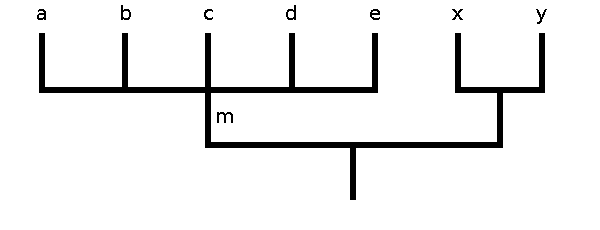
\includegraphics[scale=.5]{images/jar-example.pdf}\\
   \caption{initial tree}\label{jarInitialTree}
\end{figure}
The following figures are from JAR's \href{https://rawgit.com/OpenTreeOfLife/reference-taxonomy/registry/registry/doc/scenarios.html}{scenarios web page}.
The starting point is shown in Figure \ref{jarInitialTree} where
$m$ denotes a node that we want to bookmark.
JAR works through an example in which his sampling proposal
  initially defines a registration: \registration{m}{c,d,e}{x,y} where the
  first set is the inclusion set, and the second set is the exclusion set.
We can contrast this with a MRCA designation \mrcaDesig{m}{a}{b}.

\subsubsection{Resolutions}
\begin{figure}[h!]
   \centering  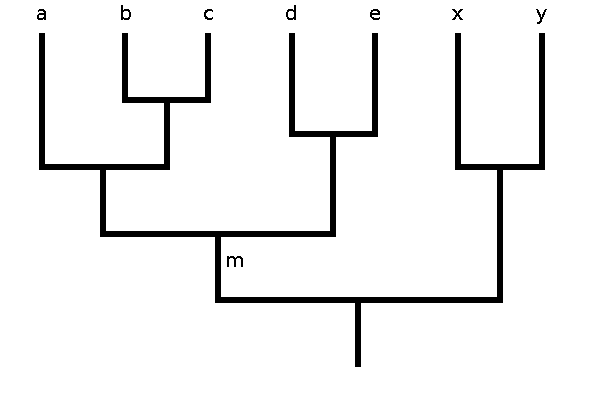
\includegraphics[scale=.5]{images/jar-unique-resolution.pdf}
   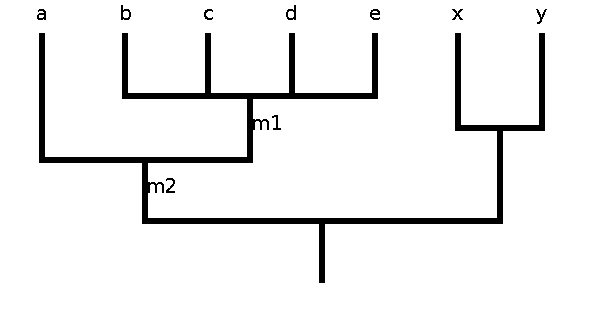
\includegraphics[scale=.5]{images/jar-ambiguous-resolution.pdf}\\
   \put{(A)\hskip 15em (B)}\\
   \caption{Two resolutions of the polytomy}\label{jarResolution1}
\end{figure}
Consider the case of a synthetic tree update that shows on of the resolutions
shown in Figure \ref{jarResolution1}.
In resolution \ref{jarResolution1}A $r(m)$ points unambiguously to the corresponding
  resolved node, but if resolution \ref{jarResolution1}B were produced
  then $r(m)$ would map to the 2 nodes marked $m1$ and $m2$
  in the new tree.
It is an open question how to deal with this ambiguity.
JAR's doc discusses using metadata, a MRCA or most inclusive ancestor procedure, or prompting the user.
$m(m)$ would resolve to a node in both cases, of course.
However, in \ref{jarResolution1}A it would resolve to the MRCA of $a,b,c$ which is not the corresponding
  node.

\subsection{Dissolution of the original monophyletic group}
\begin{figure}[h]
   \centering  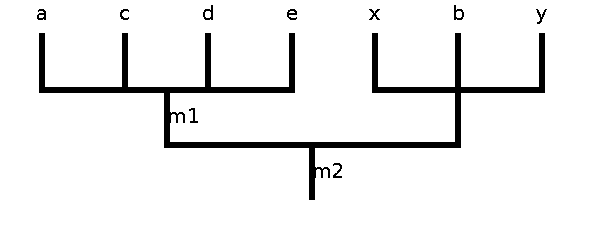
\includegraphics[scale=.5]{images/jar-false-positive.pdf}
   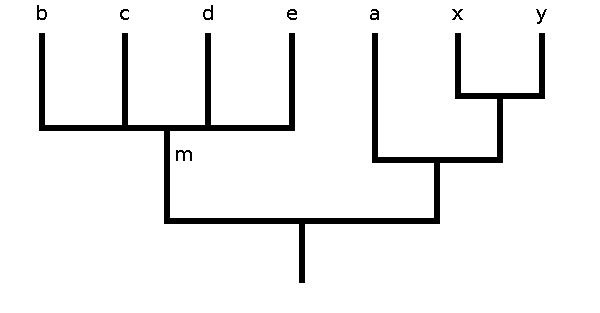
\includegraphics[scale=.5]{images/jar-relocation.pdf}
   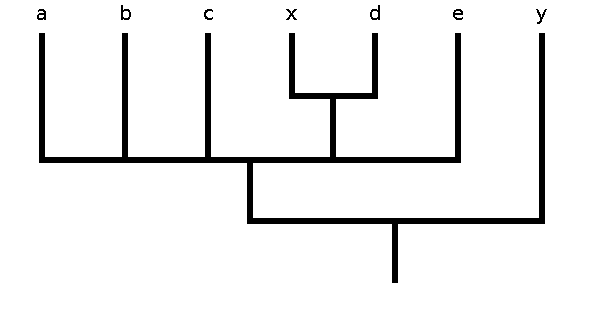
\includegraphics[scale=.5]{images/jar-no-resolution.pdf}\\
   \put{\hskip 2em(A)\hskip 12em (B)\hskip 14em (C)}\\
   \caption{3 examples of trees in which the original clade $m$ is not recovered}\label{jarDissolutionOfM}
\end{figure}
If a new version of the synthetic tree does not find the original members
  $m$ to be a clade, then the behavior of the registration system depends on
  whether or not the taxa that have ``moved away'' are among the sampled taxa
  (or whether they are paraphyletic with respect to taxa mentioned in the 
  exclude statement).
In case \ref{jarDissolutionOfM}A the $r(m)$ would no refer to the node labelled $m1$,
  despite the fact that it lacks $b$ (because $b$ was not chosen as a sampled include taxon).
In case \ref{jarDissolutionOfM}B the node labelled $m$ would be identified by $r(m)$.
In case \ref{jarDissolutionOfM}C the registration $r(m)$ would fail to map.

\subsection{Gain or loss of taxa}
\begin{figure}[h!]
   \centering  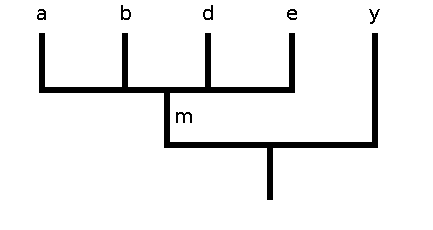
\includegraphics[scale=.5]{images/jar-sample-loss.pdf}
   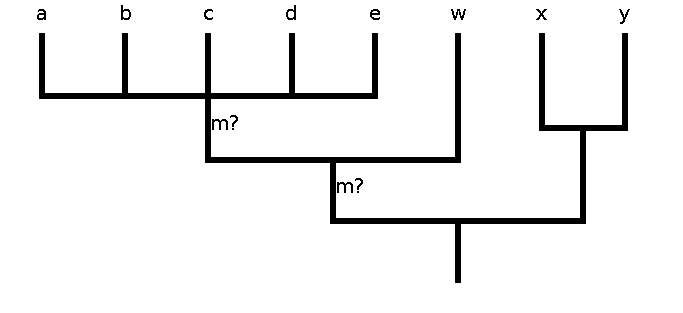
\includegraphics[scale=.5]{images/jar-new-taxon.pdf}\\
   \put{(A)\hskip 15em (B)}\\
   \caption{A tree that lacks $c$, and one that has a new leaf, $w$.}\label{jarGainLoss}
\end{figure}
The registration system is not too sensitive to taxon loss (assuming the number of sampled inclusions is not too small).
Addition of a new taxon ($w$ Figure \ref{jarGainLoss}B) results in ambiguity in this
  case.
This would be the same result if $w$ existed outside of $m$ in the original tree, but 
  was not selected as a member of the exclusion set.

\subsection{Summary of JAR scenarios}
\subsubsection{Biologists expected behavior}
If we define the ideal behavior as:
  ``Imagine that I showed the initial tree to a competent systematist
  and asked him/her
  to find the node that corresponds to $m$ in the following trees.''
I think that answers would be:\\
\begin{table}[h]
\centering
\begin{tabular}{r|c|c|c}
Case & Biologist & $r(m)$ & $m(m)$ \\
\hline
\ref{jarResolution1}A & $m$ & m & child of $m$ \\
\ref{jarResolution1}B & $m2$ & ambig. & $m2$ \\
\ref{jarDissolutionOfM}A & NA & $m1$ & root \\
\ref{jarDissolutionOfM}B & NA & $m$ & root \\
\ref{jarDissolutionOfM}C & NA & NA & non-root internal \\
\ref{jarGainLoss}A & $m^{\ast}$ & $m$ & $m$ \\
\ref{jarGainLoss}B & $m$ & ambig & tipward `$m?$' \\
\hline
\end{tabular}
\end{table}
Note that the table is not intended to show the frequency of the different scenarios.
Presumably, resolution will be the most common case.

\subsubsection{sampled registry proposal}
I don't disagree with JAR's statement (on the scenarios page): ``If the inclusion and exclusion sets are made apparent to users, and expectations are set correctly, this should be a pretty strong system$\ldots$''
However, I do think that ways that the system deviates from biologists
  expectation are a bit hard summarize to someone who does not understand the system.
Sometimes the registration-based mapping is ambiguous in cases in which biologists
  would say there is no ambiguity, and sometimes it maps when a biologist would say 
  this tree does not show that group.''
So it is not a matter of telling the users something direct like
  ``we use a stricter definition of `this group' than you may be expecting, here is why...''

Very few users will want to learn the system, and even if you understand the 
  system it would take quite a bit of coding to make the inclusion and exclusions apparent to users in a friendly way.

It could be done, but it sounds like a lot of work, and one that will be confusing to
  most users.

\subsubsection{MRCA proposal}

\section{Conclusions}
\subsection{We probably need IDs for names}
The \fragileOTUMapping argues for either
\begin{compactenum}
  \item a fixed association between names and OTT IDs whenever possible, or
  \item a much more sophisticated UI for OTU mapping that allows for mapping
    to a taxon concept (which would presumably also entail allowing curators to
    register new taxon concepts on the fly)
\end{compactenum}
The latter route would require significant UI development, so 
  it does not sound like a short-term solution.

I think that we only fill in the {\tt uniqname} in the taxonomy if 
  a name is known to be a homonym.
If OTT IDs are not attached to names, and a name is discovered to be a homonym
  in a future version of OTT,
  any record (e.g. a study in phylesystem) that stores just the OTT
  taxon name will be in danger of holding an ambiguous way of recognizing the
  mapped name.
We'd be able to sort these cases out by looking through old versions of OTT, but
  that seems like a big headache to avoid the obvious solution: establish some
  unique identifier to the names.


\bibliography{otcetera}
\end{document}



%%%%%%%%%%%%%%%%%%%%%%%
%  Cruft
Whenever a new version of OTT is produced, we sweep over the nodes of
  the tree of OTT and map all of the registrations to the internal nodes of OTT.
  \item For any internal node in OTT, $Z$, the smasher code will have a
    plausible name for that taxon {\em Ab} (\mthcomment{I think. At least I think
    that most of smasher is based on name matching}).
    \begin{compactenum}
      \item if the {\em Ab} was in a previous version of OTT, then it should
        have a registration. Let us call the registration ID $123$, for the sake of explaining this example:
        \begin{compactenum}
          \item if registration $123$ maps uniquely to node $Z$, then we do not
          then we call the node in OTT {\em Ab} and its OTT ID becomes $123$.
          \item if registration $123$ doesnode $Z$ is one of several nodes that map to $123$
        \end{compactenum}
    \end{compactenum}